\section{Fit of a constant}
\Large 
Example: Averaging of different measurements 
$a_i \pm \sigma_i$ of an observable $a$ (e.g. $a = \alpha_s(m_Z)$)
\[ \chi^2 = \Sigma_i^n \frac{ (a_i - a)^2}{\sigma_i^2} \]

``Idiot'' example of one single measurement $a_1 \pm \sigma_1$:
\[ \chi^2 = \frac{ (a_1 - a)^2}{\sigma_1^2} \]
\[Min. \chi^2: \quad \frac{d \chi^2}{da} = \; 
\rightarrow \; \mbox{Estimated value}\quad
\hat{a} = a_1; \; \sigma_{\hat{a}} = \sigma_1 \]
%
Probability density $p$ for true value of $a$ ({\em inverse probability}):
\[ p \sim e^{-\chi^2/2} = 
e^{- \frac{(a - \hat{a})^2}{2\sigma_{\hat{a}}^2}} \]
%
Important relation:
\[ \sigma_{\hat{a}} = \left[ -\frac{d\chi^2}{da^2} \right]^{-1/2}
\]

\begin{figure}[h]
\unitlength1cm
  \begin{picture}(8,7.)
    \put(0.,0.){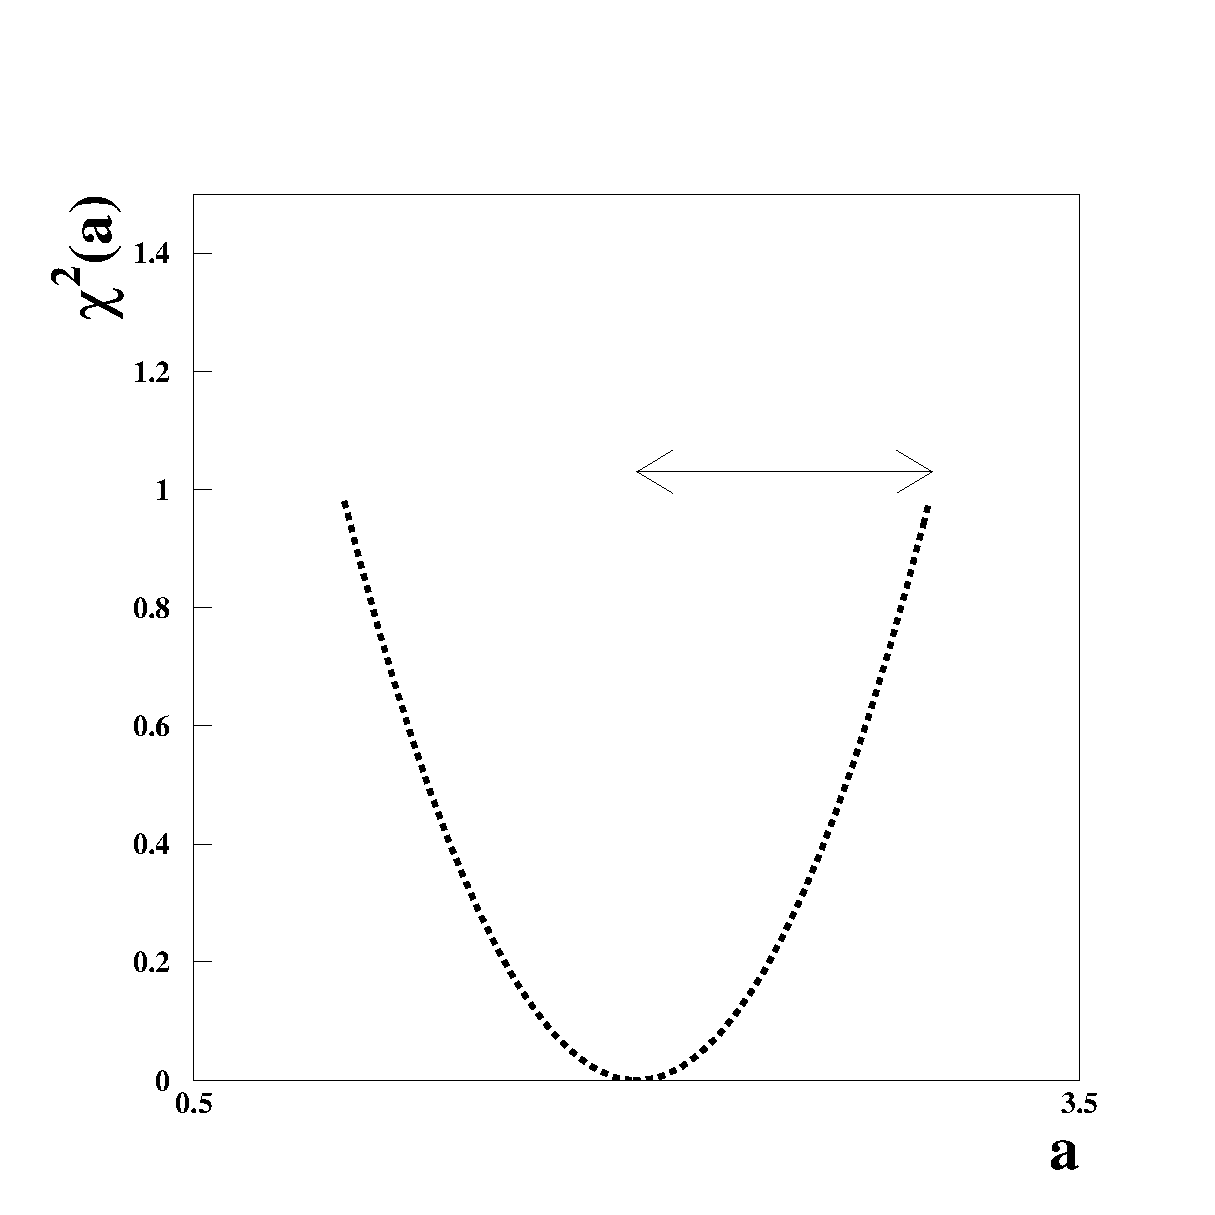
\epsfig{file=feynman/chisqp1.epsi,width=8.cm}}
    \put(8.,5.){\LARGE $\chi^2(\hat{a}+\sigma_{\hat{a}}) = 1$}
\end{picture}
\end{figure}
